\chapter{Limits and Continuity}

\section{Limits}\label{sec:limits}

Limits are a fundamental concept in calculus that describe the behavior of a function as its input 
approaches a certain value. We will not consider the rigorous definition of a limit here, but 
rather focus on the intuititive understanding of limits and how to compute them.

\begin{definition}[Limit of a Function]
    The \textit{limit} of a function $f(x)$ as $x$ approaches a value $c$ is the value that $f(x)$ approaches
    as $x$ gets closer and closer to $c$. This is denoted as:
    \begin{equation*}
        \lim_{x \to c} f(x) = L
    \end{equation*}
    where $L$ is the value that $f(x)$ approaches as $x$ approaches $c$.
\end{definition}

Now, this is a rather abstract definition. To understand it better, let us consider an example:
\begin{eg}
    Consider the function $f(x) = \frac{x^2 - 1}{x - 1}$. We want to find the limit of $f(x)$ as $x$ approaches 1:
    \begin{equation*}
        \lim_{x \to 1} \frac{x^2 - 1}{x - 1}
    \end{equation*}
    If we directly substitute $x = 1$ into the function, we get:
    \begin{equation*}
        f(1) = \frac{1^2 - 1}{1 - 1} = \frac{0}{0}
    \end{equation*}
    which is undefined. Instead, let's consider what happens to the function when it is very close to 1.
    Let's consider $x=1.1$:
    \begin{equation*}
        f(1.1) = \frac{(1.1)^2 - 1}{1.1 - 1} = \frac{0.21}{0.1} = 2.1
    \end{equation*}
    What if we got even closer? Let's try $x=1.01$:
    \begin{equation*}
        f(1.01) = \frac{(1.01)^2 - 1}{1.01 - 1} = \frac{0.0201}{0.01} = 2.01
    \end{equation*}
    And even closer, $x=1.001$:
    \begin{equation*}
        f(1.001) = \frac{(1.001)^2 - 1}{1.001 - 1} = \frac{0.002001}{0.001} = 2.001
    \end{equation*}
    We can see a pattern here: as $x$ gets closer and closer to 1, $f(x)$ gets closer and closer to 2. We conclude that 
    \begin{equation*}
        \lim_{x \to 1} \frac{x^2 - 1}{x - 1} = 2
    \end{equation*}
    Out loud, we would say: "The limit of $f(x)$ as $x$ approaches 1 is 2."
    We have considered values of $x$ that are slightly greater than 1 (i.e. we approach 1 from the right on a graph). 
    Try considering values of $x$ that are slightly less than 1 (i.e. approach 1 from the left on a graph) to verify that the limit is indeed 2.
\end{eg}

\begin{definition}[Existence of a Limit]
    We say that the limit of a function $f(x)$ as $x$ approaches $c$ \textit{exists} if the left-hand limit
    and right-hand limit are equal. That is:
    \begin{equation*}
        \lim_{x \to c^-} f(x) = \lim_{x \to c^+} f(x) = L
    \end{equation*}
    where $L$ is the value that $f(x)$ approaches as $x$ approaches $c$. In this case, we write:
    \begin{equation*}
        \lim_{x \to c} f(x) = L
    \end{equation*}
\end{definition}

\begin{notation}
    The notation $\lim_{x \to c^-} f(x)$ denotes the \textit{left-hand limit} of $f(x)$ as $x$ approaches $c$ from values less than $c$.
    The notation $\lim_{x \to c^+} f(x)$ denotes the \textit{right-hand limit} of $f(x)$ as $x$ approaches $c$ from values greater than $c$.
\end{notation}

\begin{eg}[Non-existent Limit]
    Consider the function $f(x)$ defined as:
    \begin{equation*}
        f(x) = 
        \begin{cases} 
            2 & \text{if } x < 1 \\
            3 & \text{if } x \geq 1 
        \end{cases}
    \end{equation*}
    We want to find the limit of $f(x)$ as $x$ approaches 1:
    \begin{equation*}
        \lim_{x \to 1} f(x)
    \end{equation*}
    Let's consider the left-hand limit:
    \begin{equation*}
        \lim_{x \to 1^-} f(x) = 2
    \end{equation*}
    Now, let's consider the right-hand limit:
    \begin{equation*}
        \lim_{x \to 1^+} f(x) = 3
    \end{equation*}
    Since the left-hand limit (2) and right-hand limit (3) are not equal, we conclude that the limit of $f(x)$ as $x$ approaches 1 does not exist.
    Perhaps a graphical representation of this function would help illustrate this concept better.
    \begin{figure}[H]
    \centering
      \begin{tikzpicture}
          \begin{axis}[
              axis lines = middle,
              xlabel = $x$,
              ylabel = {$f(x)$},
              ymin=0, ymax=4,
              xmin=0, xmax=2,
              xtick={1},
              ytick={2,3},
              yticklabels={2,3},
              domain=0:2,
              samples=100,
              width=10cm,
              height=6cm,
          ]
              % Left piece: y=2 for x in [0, just before 1)
              \addplot[blue, thick, domain=0:0.98, samples=2] {2};
              % Open circle at (1,2) with blue stroke, no fill
              \addplot[blue, only marks, mark=o, mark options={scale=1.2,draw=blue,fill=white,line width=1.2pt}] coordinates {(1,2)};
              % Right piece: y=3 for x in [1,2]
              \addplot[red, thick, domain=1:2, samples=2] {3};
              % Solid dot at (1,3)
              \addplot[red, only marks, mark=*, mark options={scale=1.2}] coordinates {(1,3)};
          \end{axis}
      \end{tikzpicture}
      \caption{Graph of the piecewise function $f(x)$}
  \end{figure}

Clearly, from the left side (blue), the function approaches 2, while from the right side (red), 
the function approaches 3. This limit does not exist. Note that we have used an open circle on the left side at $x=1$ to indicate that the function 
does not include that poin (i.e. $f(x) = 2$ when $x<1$, but not when $x=1$).
\end{eg}

\section{Continuity}

Continuity of a function is a fairly intuitive concept. A discontinuous function is
one which contains a `jump' or `break' in its graph. Keep this intuition in mind as 
we define continuity more formally.

\begin{definition}[Continuity at a Point]\label{def:continuity}
    A function $f(x)$ is said to be \textit{continuous} at a point $x = c$ if the following three conditions are met:
    \begin{enumerate}
        \item $f(c)$ is defined (i.e. $c$ is in the domain of $f$, and not $f(c) \rightarrow \infty$).
        \item The limit of $f(x)$ as $x$ approaches $c$ exists.
        \item The limit of $f(x)$ as $x$ approaches $c$ is equal to $f(c)$:
        \begin{equation*}
            \lim_{x \to c} f(x) = f(c)
        \end{equation*}
    \end{enumerate}
\end{definition}

\begin{definition}[Continuity on an Interval]
    A function $f(x)$ is said to be \textit{continuous} on an interval $a \le x \le b$ if it is continuous at every point $x$ in the interval (i.e.
    every point between $a$ and $b$, inclusive).
\end{definition}

\begin{definition}[Continuous Function]
    A function $f(x)$ is said to be a \textit{continuous function} if it is continuous at every point in its domain.
    A function which is not continuous is called \textit{discontinuous}.
\end{definition}

While the \hyperref[def:continuity]{rigorous definition of continuity} is somewhat complex, deciding whether a function
is continuous is often just a matter of determining whether there are any `jumps' or `breaks' in its graph. A function also 
becomes discontinuous if there is a vertical asymptote (i.e. the function approaches infinity at some point). These 
are the phenomena we look out for when determining whether a function is continuous.

\begin{exercise}[Easy]
    Determine whether the function $f(x)$ defined as:
    \begin{equation}\label{eq:continuity-ex1}
        f(x) = 
        \begin{cases} 
            x^2 & \text{if } x \neq 2 \\
            5 & \text{if } x = 2 
        \end{cases}
    \end{equation}
    is continuous at $x=2$.
\end{exercise}
\begin{answer}
    To determine whether $f(x)$ is continuous at $x=2$, we will check the three conditions from the definition of continuity:
    \newline\newline
    \textbf{Condition 1:} $f(2)$ is defined. From the definition of $f(x)$, we see that $f(2) = 5$. Therefore, condition 1 is satisfied.
    \newline\newline
    \textbf{Condition 2:} The limit of $f(x)$ as $x$ approaches 2 exists. We need to compute:
    \begin{equation*}
        \lim_{x \to 2} f(x)
    \end{equation*}
    Since $f(x) = x^2$ for all $x \neq 2$, we can compute the limit using this expression:
    \begin{equation*}
        \lim_{x \to 2} x^2 = 2^2 = 4
    \end{equation*}
    Any polynomial function is continuous everywhere, so we can compute the limit by direct substitution. 
    Therefore, condition 2 is satisfied.
    \newline\newline
    \textbf{Condition 3:} The limit of $f(x)$ as $x$ approaches 2 is equal to $f(2)$. We have:
    \begin{equation*}
        \lim_{x \to 2} f(x) = 4
    \end{equation*}
    and
    \begin{equation*}
        f(2) = 5
    \end{equation*}
    Since $4 \neq 5$, condition 3 is not satisfied.
    \newline\newline
    Since condition 3 is not satisfied, we conclude that the function $f(x)$ is not continuous at $x=2$.
    \begin{figure}[H]
    \centering
    \begin{tikzpicture}
      \begin{axis}[
          axis lines = middle,
          xlabel = $x$,
          ylabel = {$f(x)$},
          domain=0:4,
          samples=100,
          ymin=0, ymax=8,
          xtick=\empty,
          ytick=\empty,
          ytick={4,5},
          yticklabels={$4$,$5$},
          xtick={2},
          grid=none,
          width=10cm,
          height=6cm
        ]
        % Plot y = x^2 except at x=2
        \addplot [red, thick, domain=0:1.98] {x^2};
        \addplot [red, thick, domain=2.02:4] {x^2};
        % Open circle at (2,4)
        \addplot [red, only marks, mark=o, mark options={scale=1.2,draw=red,fill=white,line width=1.2pt}] coordinates {(2,4)};
        % Solid dot at (2,5)
        \addplot [red, only marks, mark=*, mark options={scale=1.2}] coordinates {(2,5)};
      \end{axis}
    \end{tikzpicture}
    \caption{Graph of equation \ref{eq:continuity-ex1}}
\end{figure}
\end{answer}

% Plot of f(x) = (x+2)/(x+1) with vertical and horizontal asymptotes

\section{Asymptotes}

Asymptotes are lines that a graph approaches but never touches. 
There are three types of asymptotes: vertical, horizontal, and oblique (slant).

\begin{definition}[Vertical Asymptote]
    A vertical asymptote is a vertical line $x = a$ where the function $f(x)$ approaches infinity (or negative infinity) as $x$ approaches $a$. 
    This typically occurs at points where the function is undefined, such as points of division by zero.
\end{definition}

\begin{definition}[Horizontal Asymptote]
    A horizontal asymptote is a horizontal line $y = b$ where the function $f(x)$ approaches $b$ as $x$ approaches positive or negative infinity. 
    This indicates the behavior of the function as it extends towards the extremes of the $x$-axis.
\end{definition}

\begin{definition}[Oblique Asymptote]
    An oblique (or slant) asymptote is a diagonal line $y = mx + b$ where the function $f(x)$ approaches this line as $x$ approaches positive or negative infinity. 
    Oblique asymptotes occur when the degree of the numerator is one greater than the degree of the denominator in a rational function.
\end{definition}

% draw me a 3x1 set of graphs showing vertical, horizontal, and oblique asymptotes using tikz and pgfplots
\begin{figure}[H]
    \centering
    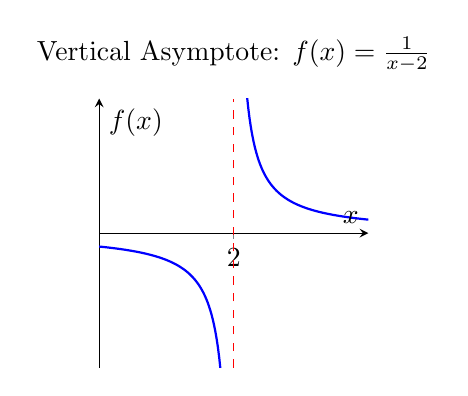
\begin{tikzpicture}
        \begin{axis}[
            title={Vertical Asymptote: $f(x) = \frac{1}{x-2}$},
            axis lines = middle,
            xlabel = $x$,
            ylabel = {$f(x)$},
            ymin=-5, ymax=5,
            xmin=0, xmax=4,
            xtick={2},
            ytick=\empty,
            width=5cm,
            height=5cm,
        ]
            \addplot[blue, thick, domain=0:1.9, samples=100] {1/(x-2)};
            \addplot[blue, thick, domain=2.1:4, samples=100] {1/(x-2)};
            \addplot[dashed, red] coordinates {(2,-5) (2,5)};
        \end{axis}
    \end{tikzpicture}
    \hspace{1cm}
    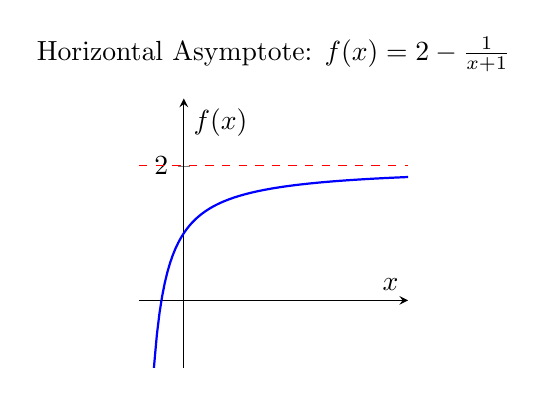
\begin{tikzpicture}
        \begin{axis}[
            title={Horizontal Asymptote: $f(x) = 2 - \frac{1}{x+1}$},
            axis lines = middle,
            xlabel = $x$,
            ylabel = {$f(x)$},
            ymin=-1, ymax=3,
            xmin=-1, xmax=5,
            ytick={2},
            yticklabels={$2$},
            xtick=\empty,
            width=5cm,
            height=5cm,
        ]
            \addplot[blue, thick, domain=-0.9:5, samples=100] {2 - 1/(x+1)};
            \addplot[dashed, red] coordinates {(-1,2) (5,2)};
        \end{axis}
    \end{tikzpicture}
    \hspace{1cm}
    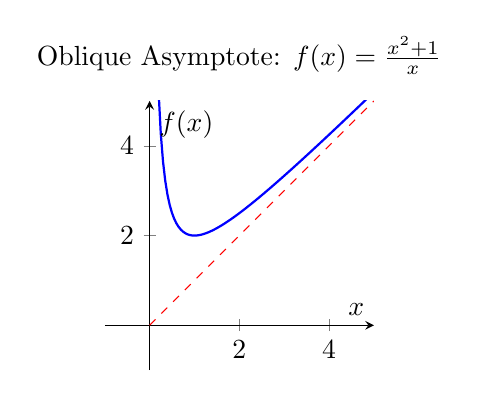
\begin{tikzpicture}
        \begin{axis}[
            title={Oblique Asymptote: $f(x) = \frac{x^2 + 1}{x}$},
            axis lines = middle,
            xlabel = $x$,
            ylabel = {$f(x)$},
            ymin=-1, ymax=5,
            xmin=-1, xmax=5,
            width=5cm,
            height=5cm,
        ]
            \addplot[blue, thick, domain=0.1:5, samples=100] {(x^2 + 1)/x};
            % Correct oblique asymptote: y = x
            \addplot[dashed, red, domain=0:5] {x};
        \end{axis}
    \end{tikzpicture}
    \caption{Examples of Vertical, Horizontal, and Oblique Asymptotes}
    \label{fig:asymptotes}
\end{figure}

A \textit{vertical asymptote} typically occurs when the denominator of a function approaches zero
(as long as the numerator does not also approach zero). At this point, we are dividing a finite number by 
zero, giving us an infinite result. In the example above, the function $f(x) = \frac{1}{x-2}$ has a vertical asymptote at $x=2$,
since the denominator becomes zero at this point. 

A \textit{horizontal asymptote} is slightly different. The function above, 
$f(x) = 2 - \frac{1}{x+1}$, can never be exactly equal to 2, because 
the fractional term can never be zero (a fraction can only ever be zero if its numerator
is zero). However, as $x$ becomes very large (either positively or negatively), the fractional term 
becomes very small, and the function approaches 2. Therefore, $y=2$ is a horizontal asymptote of this function.
The hardest part about horizontal asymptotes is writing the function in a form similar to the above.

\begin{exercise}
    Determine the vertical and horizontal asymptotes of the function:
    \begin{equation*}
        f(x) = \frac{x+2}{x+1}
    \end{equation*}
\end{exercise}
\begin{answer}
    We will first solve for the vertical asymptote and then for the horinzontal asymptote. 
    \newline\newline
    \textbf{Vertical Asymptote:} To find the vertical asymptote, we need to determine what value of $x$
    makes the denominator zero. Setting the denominator equal to zero, we have:
    \begin{equation*}
        x + 1 = 0
    \end{equation*}
    Solving for $x$, we find:
    \begin{equation*}
        x = -1
    \end{equation*}
    Therefore, the vertical asymptote is at $x = -1$.
    \newline\newline
    \textbf{Horizontal Asymptote:} To find the horizontal asymptote, we first need to rewrite the function 
    in the appropriate form. This means that the numerator must not be dependent on x. 
    We do this by considering the numerator as some multiple of the denominator, plus a constant:
    \begin{align*}
        f(x) &= \frac{x+2}{x+1} \\
             &= \frac{(x+1) + 1}{x+1} \\
             &= \frac{x+1}{x+1} + \frac{1}{x+1} \\
             &= 1 + \frac{1}{x+1}
    \end{align*}
    Now, we can see that as $x$ approaches positive or negative infinity, the fractional term approaches zero. 
    Therefore, the function approaches 1. Thus, the horizontal asymptote is at $y = 1$. The horizontal asymptote
    is always the multiple of the denominator that gives us the numerator when we rewrite the function.
    \begin{figure}[H]
    \centering
    \begin{tikzpicture}
        \begin{axis}[
            axis lines = middle,
            xlabel = $x$,
            ylabel = {$f(x)$},
            domain=-4:4,
            samples=200,
            ymin=-4, ymax=4,
            xmin=-4, xmax=4,
            xtick={-1},
            ytick={1},
            yticklabels={$1$},
            grid=none,
            width=10cm,
            height=6cm
        ]
            % Plot f(x) = (x+2)/(x+1), avoiding x=-1
            \addplot[red, thick, domain=-4:-1.05] {(x+2)/(x+1)};
            \addplot[red, thick, domain=-0.95:4] {(x+2)/(x+1)};
            % Vertical asymptote x=-1
            \addplot[dashed, red] coordinates {(-1,-4) (-1,4)};
            % Horizontal asymptote y=1
            \addplot[dashed, red, domain=-4:4] {1};
        \end{axis}
    \end{tikzpicture}
    \caption{Graph of $f(x) = \frac{x+2}{x+1}$ with vertical asymptote $x=-1$ and horizontal asymptote $y=1$}
\end{figure}
\end{answer}

\textit{Oblique asymptotes} are less common, but the process for finding them
is similar to that for horizontal asymptotes. Rather than finding an constant
multiple of the denominator, we need to find a linear function of $x$ (i.e. $mx + b$) such 
that when we rewrite the function, the numerator can be written as this linear function
multiplied by the denominator, plus a remainder. The oblique asymptote is then this linear function.
An example is instructive here. 

\begin{exercise}
    Find the oblique asymptote of the function:
    \begin{equation*}
        f(x) = \frac{2x^2 + 1}{x}
    \end{equation*}
\end{exercise}
\begin{answer}
    This function clearly has a vertical asymptote at $x=0$ (denominator is zero).
    It does not have a horizontal asymptote, since the degree of the numerator is greater than
    that of the denominator. In this case, we look for an oblique asymptote.
    We use the same trick as we used for the horizontal asymptote, but rather than a constant multiple,
    we look for a linear function $mx + b$ such that:
    \begin{equation*}
        2x^2 + 1 = (mx + b)(x) + R
    \end{equation*}
    where $R$ is some remainder (which may be zero).
    In this case, we can see that $m=2$ and $b=0$ works, since:
    \begin{align*}
        f(x) &= \frac{2x^2 + 1}{x} \\
             &= \frac{(2x)(x) + 1}{x} \\
             &= \frac{(2x)(x)}{x} + \frac{1}{x} \\
             &= 2x + \frac{1}{x}
    \end{align*}
    Therefore, the oblique asymptote is $y = 2x$.
    \begin{figure}[H]
    \centering
    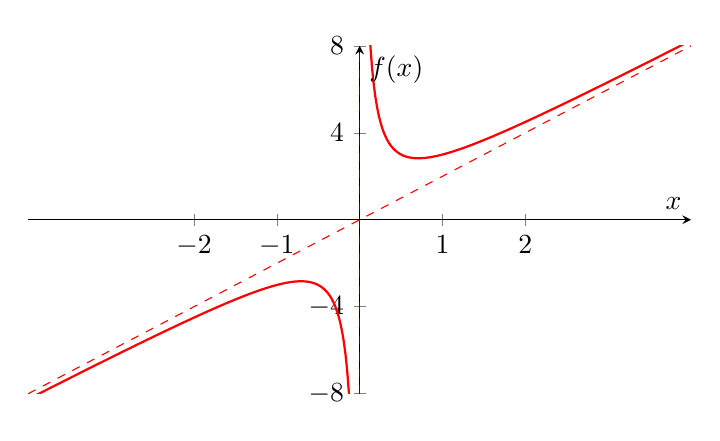
\begin{tikzpicture}
        \begin{axis}[
            axis lines = middle,
            xlabel = $x$,
            ylabel = {$f(x)$},
            domain=-4:4,
            samples=200,
            ymin=-8, ymax=8,
            xmin=-4, xmax=4,
            xtick={-2,-1,0,1,2},
            ytick={-8,-4,0,4,8},
            grid=none,
            width=10cm,
            height=6cm
        ]
            % Plot f(x) = (2x^2 + 1)/x, avoiding x=0
            \addplot[red, thick, domain=-4:-0.05] {(2*x^2 + 1)/x};
            \addplot[red, thick, domain=0.05:4] {(2*x^2 + 1)/x};
            % Vertical asymptote x=0
            \addplot[dashed, blue] coordinates {(0,-8) (0,8)};
            % Oblique asymptote y=2x
            \addplot[dashed, red, domain=-4:4] {2*x};
        \end{axis}
    \end{tikzpicture}
    \caption{Graph of $f(x) = \frac{2x^2 + 1}{x}$ with vertical asymptote $x=0$ and oblique asymptote $y=2x$}
\end{figure}
\end{answer}